%no borrar PREAMBULO
\documentclass[12pt]{article}

\usepackage[top=3.5 cm, bottom=2.5  cm, left=3 cm, right=3 cm]{geometry}
\usepackage{fancyhdr}
\pagestyle{fancy}

\usepackage[hidelinks]{hyperref} %esta opción saca las cajas de colores de los hiperlinks

\fancyfoot[C]{\thepage }  %numera las páginas

\usepackage[utf8]{inputenc}

\usepackage{amsmath,amsfonts,amssymb}
\usepackage{xcolor}
\usepackage{fancyvrb}
\newcommand\verbbf[1]{\textcolor[rgb]{0,0,1}}%comando para colorear el texto en verbatim
%\linespread{1} %por si queremos achicar el espacio entre lineas

\usepackage{tabularx,booktabs}
\usepackage{graphicx}
\usepackage{float} %para que las figuras puedan ponerse en cualquier lado

\usepackage{subcaption}
\usepackage{layout}
\usepackage{multicol}  %para escribir en columnnas 
\usepackage{float}
\usepackage{textcomp}
\usepackage{natbib}
\usepackage{tikz}
\usepackage{multirow} %para cambiar el alto de una fila en una tabla
\tikzset{
  connect/.style = { dashed, gray }
}
\usepackage{pgfplots}
\pgfplotsset{compat=1.8}
\usepackage[english ,spanish]{babel}
\usepackage{latexsym}
\usepackage{verbatim}

%\usepackage{alltt}
\usepackage{indentfirst}

\usepackage[flushmargin]{footmisc} %para alinear las notas de página

\usepackage{url}
\usepackage{advdate}
\usepackage{wrapfig}
\usepackage{amsthm}
\usepackage[inline]{enumitem} %para hacer listas en una linea, los mismos comandos con *
\newtheorem*{myteo}{Teorema} % la * es para no numerarlos
\newtheorem*{myexample}{Ejemplo}
\newtheorem*{myprop}{Proposición}
\newtheorem*{mylem}{Lema}
\theoremstyle{definition}
\newtheorem*{mydef}{Definición}
\newtheorem{ejer}{Ejercicio}
\newtheorem*{mydefs}{Definiciones}
\theoremstyle{remark}
\newtheorem*{myobs}{Observación}


\renewcommand{\baselinestretch}{1}  %interlineado

\addto\captionsspanish{%
  \renewcommand{\figurename}{Figura}%
}

\newcommand\myText[1]{\text{\scriptsize\tabular[t]{@{}l@{}}#1\endtabular}}
\addto\captionsspanish{%
  \renewcommand{\tablename}{Tabla}%
}

\def \ds {\displaystyle} %define un comando abreviado  
\def\com{“R”}

\usepackage{hyperref}%para referencias de internet con link!
\newcommand*{\fullref}[1]{\hyperref[{#1}]{ \nameref*{#1}}}
%comando \fullref para que ademas del número de capitulo, sección etc. escriba el título del capitulo, sección o lo que sea a lo que estamos haciendo referencia

\newcommand\comentario[1]{\textcolor{red}{#1}}%comentarios en el pdf

\interfootnotelinepenalty=10000 %previene que se pasen a otra página las notas de pie
\raggedbottom 
\addtolength{\topskip}{0pt plus 10pt}
\addtolength{\footnotesep}{0.1mm}

\VerbatimFootnotes%para poder usar Verbatim en las notas de pie

\begin{document}

\fancyhf{}
\pagestyle{fancy}
\lhead{Departamento de Matem\'{a}tica\\Universidad Nacional del Comahue}
\rhead{Matem\'{a}tica 1\\ Licenciatura en Ciencias Biol\'{o}gicas}

%HASTA ACA 

\begin{centering}
\Large{\textbf{Trabajo Práctico N° 3}}\\
\large{\textbf{Soluciones de ejercicios seleccionados}}\\
\large{\textbf{Lógica y Conjuntos}}\\
\end{centering}
\vspace{1cm}
\noindent
En este documento ofreceremos las soluciones de algunos ejercicios y problemas seleccionados de este Trabajo Práctico con explicaciones que permitan seguir el razonamiento para su resolución. Como la numeración de los ejercicios de las distintas versiones del TP pueden variar, incluimos antes de la solución, el ejercicio que se resolverá.

%n: 3,5,7,8,9,11,17, 24 y 26.
\begin{enumerate}


%1
\item \textbf{Ejercicio 1:} Determinar si las siguientes expresiones son proposiciones y cuáles no lo son. Explicar por qué.
\begin{multicols}{2}
 \begin{enumerate}
 \setlength\itemsep{0em}
        \item El sol es cuadrado.
        \item La cuchara sirve para.
        \item La mamá sirve postre.
        \item Mi bisabuela se peinó con rodete el 16 de julio de 1899.
        \item ¿Qué hora es?
        \item ¿Existe la justicia?
        \item Existe la justicia
        \item No existe la justicia
        \item $2 + 5 = 6$
        \item $2 + 5 = 7$
        \item$2 + 5 $
  \end{enumerate}
\end{multicols}
\noindent
\textbf{Solución} \\
Son proposiciones sólo si (aunque sea en teoría) se puede decir de ellas si son V o F. Por ejemplo, pensemos en el caso de la bisabuela. Quizás no tengamos manera de saber si es cierto o no, pero usó rodete (V) o no lo usó (F). Entonces es una proposición. Sólo son  proposiciones \textit{a, c, d, g, h, i} y  \textit{j}.


%3
\item \textbf{Ejercicio 3:} Dadas las siguientes proposiciones,
 \begin{multicols}{2}
 \begin{enumerate}
 \setlength\itemsep{0em}
     	\item Todos los perros son blancos.
	\item Hay mamíferos que vuelan.
	\item Existe un león que ruge.
	\item Los leones tienen melena.
	\item Hay gallinas que ponen huevos verdes.
	\item Ningún metal es líquido.
	\item Hay plantas que no se reproducen por semillas.
  \end{enumerate}
\end{multicols}
 Se pide identificar un conjunto de referencia para cada uno  y redactar las proposiciones anteriores de la forma  \textit{Todo...} o \textit{Existe...} (cuando sea necesario)(¡no es importante si las afirmaciones son verdaderas o falsas!)

Ejemplo: Todos los perros son blancos $\rightarrow$  \textit{Conjunto de referencia}: El conjunto de todos los perros que existen. \textit{Enunciado en la forma “ Todo…” }  $\rightarrow$ Todo perro es blanco.

\noindent
\textbf{Solución} \\
Primero daremos los referenciales:
 \begin{multicols}{2}
 \begin{enumerate}
 \setlength\itemsep{0em}
     	\item El conjunto de todos los perros.
	\item El conjunto de mamíferos.
	\item El conjunto de los leones.
	\item Idem anterior.
	\item El conjunto de las gallinas.
	\item El conjunto de los metales.
	\item El conjunto de las plantas.
  \end{enumerate}
\end{multicols}

Ahora escribiremos las afirmaciones usando la forma  \textit{Todo...} o \textit{Existe...} 
\begin{multicols}{2}

 \begin{enumerate}
 \setlength\itemsep{0em}
     	\item Todo perro es blanco (o como estaba originalmente). 
	\item Existe (al menos) un mamífero que vuela.
	\item Existe un león que ruge.
	\item Todo león tiene melena.
	\item Existe una gallina (o Existen gallinas) que pone huevos verdes.
	\item Todo metal no es líquido.
	\item Existe una planta (o Existen plantas) que no se reproduce por semillas.
  \end{enumerate}
\end{multicols}

%5
\item \textbf{Ejercicio 5:} Explicar cómo demostrarías si las afirmaciones del Ejercicio 3 son verdaderas o falsas.\\
\noindent
\textbf{Solución:} 
 \begin{enumerate}
% \setlength\itemsep{0em}
        	\item  “Todos los perros son blancos". \textbf{Falso}. Para demostrar que una afirmación con el cuantificador \textit{Todo}  es Falsa basta con mostrar un \textit{contraejemplo}. Bastará con salir a la calle y mostrar el primer perro que pase que no sea blanco. Si es Falsa la afirmación, es por que \textit{existe} al menos un perro que no es blanco.
	\item “Existe un mamífero que vuela". \textbf{Verdadero}. Para demostrar que una afirmación con el cuantificador \textit{existe}  es Verdadera basta con mostrar un \textit{ejemplo}. Bastará con salir a la calle (o al bosque) encontrar un mamífero que levante vuelo. O, en épocas de cuarentena, ir a \textit{Wikipedia} y encontrar una especie de mamíferos que tenga esta habilidad, como el murciélago. 
	\item “Existe un león que ruge". \textbf{Verdadero}. Es igual a  la anterior. Ponemos una película de la \textit{Metro Goldwiyn Mayer} y vemos que, efectivamente, existe un león que ruge.
	\item “Todo león tiene melena". \textbf{Verdadero} (supongamos). Como en cualquier caso en que que tenemos que mostrar que una afirmación con el cuantificador \textit{Todo} es verdadera, lo primero es distinguir si el conjunto al que hacemos referencia es finito o infinito. Si es infinito, estamos frites, tenemos que utilizar algún razonamiento deductivo, que nos permita mostrar la validez de la afirmación a partir de verdades que ya sabemos/conocemos/aceptamos. En el caso de conjuntos finitos, aunque sea teóricamente, tenemos la posibilidad de hacer una revisión exhaustiva de la totalidad de los elementos del conjunto y verificar que cada uno cumple con la condición que expresa la proposición. Es decir, revisando exhaustivamente, estamos viendo que  \textit{no existe} dentro del conjunto, ningún elemento que  \textit{no cumpla} con la condición. En este caso, deberíamos mirar uno por uno los leones del mundo (de nuestro referncial) y veririficar que todos tienen melena (las que no tienen son las leonas).
	\item “Existe una gallina que pone huevos verdes". Si fuera \textbf{verdadero} (lo es, doy fe, las gallinas negras ponen huevos verdes) procedemos como en el caso del león que ruge. Si fuera \textbf{falso}, en cambio, tenemos que proceder como en el ejemplo de la melena de los leones. Para mostrar que es falso que existe una gallina con esta asombrosa propiedad, deberíamos revisar gallina por gallina, y esperar que ponga un huevo, y verificar que no es verde!
	\item “Todo metal no es líquido". \textbf{Falso}. Igual que la de los perros blancos.
	\item “Existen plantas que no se reproducen por semillas". Igual que las gallinas.
  \end{enumerate}
%\end{multicols}

%7
\item \textbf{Ejercicio 7:} Considere un referencial $R$ formado por las siguientes figuras donde hay tres formas (triángulo, cuadrado y círculo), en dos tamaños (grande y pequeño) y  tres “colores” (negro, blanco y a rayas) que se muestran a continuación. Tenemos $18$ formas posibles que surgen de combinar las características forma, tamaño y color.  Ahora llamemos:
\begin{itemize}
\item A al conjunto de todas las figuras del referencial que hagan verdadera la proposición \textbf{n}: “la figura es negra”
\item B al conjunto de todas las figuras del referencial que hagan verdadera la proposición \textbf{g}: “la figura es grande” 
\end{itemize}
\begin{figure}[H]
\centering
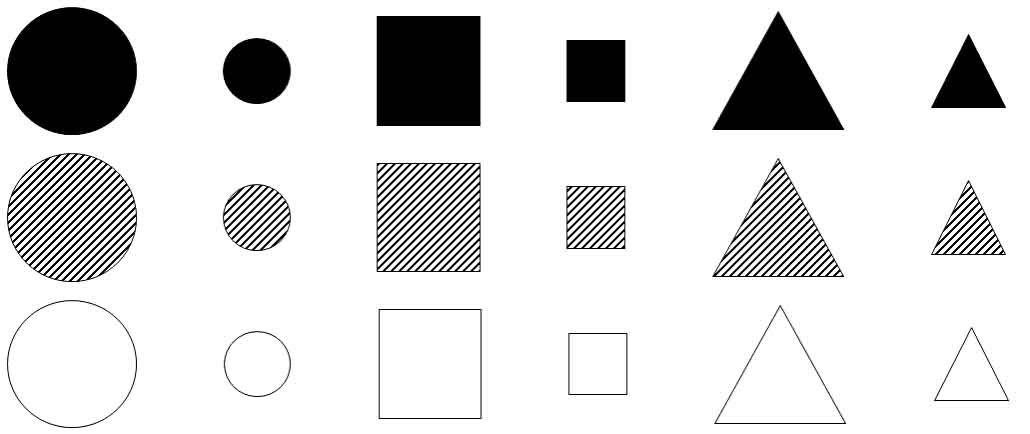
\includegraphics[width=0.7\textwidth]{TP1Fig1}
%\caption{Conjunto referencial. Las figuras se clasifican por forma, color y tamaño}
\end{figure}

\noindent
\textbf{Solución en cada ítem} 
\begin{enumerate}
\item Representar gráficamente los conjuntos A y B mediante un diagrama: 
\begin{figure}[H]
\centering
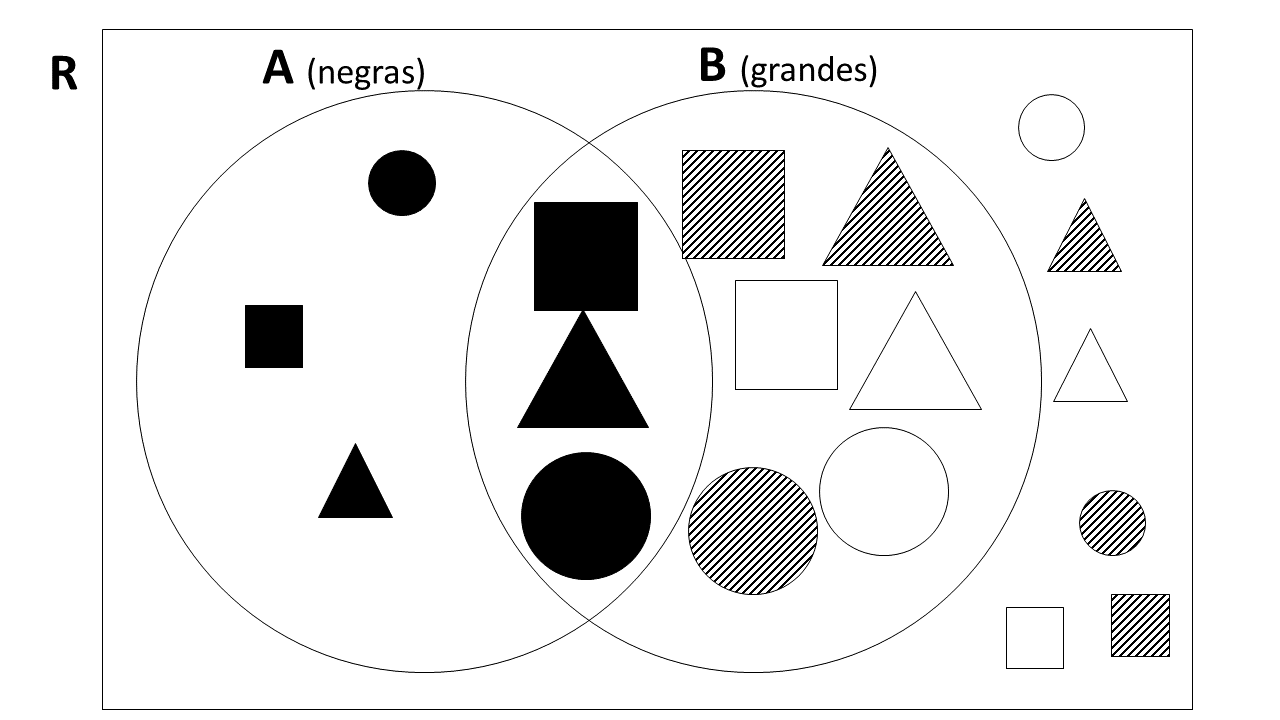
\includegraphics[width=0.5\textwidth]{7a}
\end{figure}
\item De acuerdo a esta representación, ¿qué elementos se encuentran en la región $A\cap B$?\\
\textbf{R:} Figuras que son negras y grandes a la vez.
\item Enunciar la proposición compuesta que verifican los elementos de $A\cap B$ utilizando el conectivo lógico $\wedge$.\\
\textbf{R:} $n \wedge g$: $x$ es una figura negra $\land$ x es una figura grande.
\item ¿Qué elementos se encontrarán en la región II? Escribir la proposición compuesta con el conectivo correspondiente.\\
\textbf{R:} La región II corresponde a la diferencia de conjuntos $A-B$. Son las figuras que son negras pero no son grandes. La proposición es: $n \wedge \sim g$: $x$ es una figura negra $\land$ $x$ es una figura no grande. Aún cuando en este ejemplo no hay otra cosa que grandes o pequeñas y uno podría poner $x$ es una figura negra $\land$ x es una figura pequeña, lo correcto es lo anterior.
\item ¿Qué elementos se encontrarán en la región III? Escribir la proposición compuesta con el conectivo correspondiente.\\
\textbf{R:} Análogo al anterior. La región III corresponde a la diferencia de conjuntos $B-A$. Figuras grandes que no sean negras. La proposición es: $g  \wedge \sim n$: $x$ es una figura grande $\land$ x es una figura no negra. Acá queda clara la necesidad de escribir la negación de “negra'' como “no negra'', porque esta negación incluye las opciones “rayada'' o “blanca''. 
\item ¿Qué elementos se encontrarán en la región IV? Escribir la proposición compuesta con el conectivo correspondiente.\\
\textbf{R:} La región IV corresponde al complemento de la unión de $A$ y $B$, es decir: $\overline{A\cup B}$. Son las figuras que no son ni negras ni grandes. La proposición se escribe como: $ \sim(n \vee  g)$: la figura no es negra o grande. esta afirmación es equivalente a $\sim n \wedge \sim g$: $x$ es una figura no negra $\land$ x es una figura no grande. 
\end{enumerate}



%8
\item  \textbf{Ejercicio 8:} Para el mismo referencial del ejercicio anterior, supongamos ahora que:
\begin{itemize}
\setlength\itemsep{0em}
\item A es conjunto de todas las figuras del referencial que hacen verdadera la proposición \textbf{b}: “la figura es blanca”.
\item B es conjunto de todas las figuras del referencial que hacen verdadera la proposición \textbf{t}: “la figura es triángulo”. 
\end{itemize}

\noindent
\textbf{Solución} 
Representamos gráficamente estos conjuntos mediante un diagrama de Venn como en el caso anterior:
\begin{figure}[H]
\centering
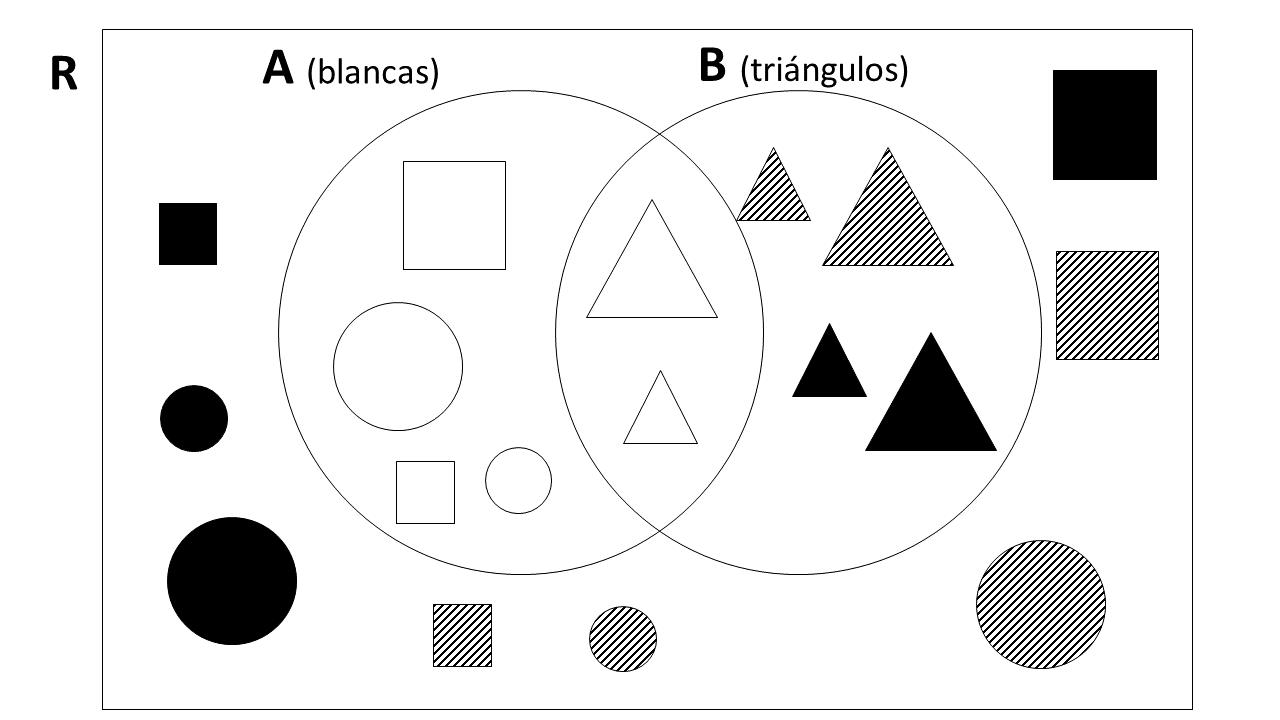
\includegraphics[width=0.5\textwidth]{8a}
\end{figure}

\begin{enumerate}
\item Enunciar, haciendo uso de conectivos lógicos, las proposiciones que hacen verdaderas las figuras que se ubican en las regiones  I, II, III y IV.\\
\textbf{R:} \\
Región I: $A\cap B$. La proposición es  $p \wedge q$: $x$ es una figura blanca y es un triángulo\\
Región II: $A- B$. La proposición es  $p \wedge \sim q$: $x$ es una figura blanca y no es un triángulo\\
Región III: $B -  A$. La proposición es  $q \wedge \sim p$: $x$ es un triángulo y no es blanco\\
Región IV:$\overline{A\cup B}$. La proposición es  $\sim p \wedge \sim q$: : $x$  no es una figura blanca o no es un triángulo (ver último punto del ejercicio anterior)\\

\item Describir las figuras del referencial R que se ubican en la unión de A y B. Enunciar la proposición compuesta que cumplen los elementos de  $A\cup B$ utilizando el conectivo lógico  $\vee$.

\textbf{R:} Los elementos de $A\cup B$  son figuras blancas o triángulos de cualquier color. La proposición es $p \vee q$: $x$  es una figura blanca o es un triángulo.

\item Si una figura no es triángulo pero está en $A\cup B$, ¿qué podemos afirmar de esa figura?\\
\textbf{R:} Si no es triángulo pero está en la unión, es cuadrado o círculo blanco.

\item Escribir algunas proposiciones compuestas utilizando el conectivo “o inclusivo” ($\vee$) y el “o excluyente” ($\veebar$) y analizar en qué casos serán verdaderas.
\textbf{R:}
\begin{itemize}
\setlength\itemsep{0em}
\item $\sim p \vee q$: la figura no es blanca o es un triángulo\\
\begin{figure}[H]
\centering
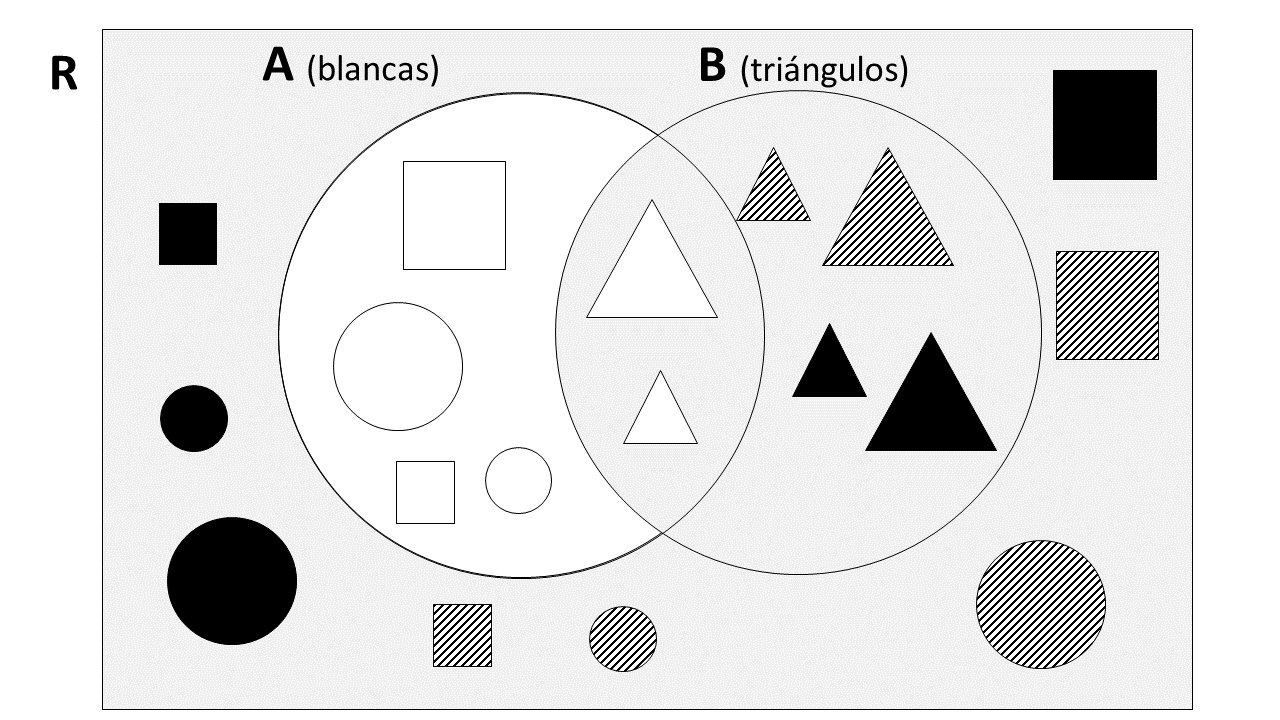
\includegraphics[width=0.5\textwidth]{9a}
\end{figure}
\item  $p \veebar q$: $x$ es una figura blanca o es un triángulo pero no un triángulo blanco. Recordar que la disyunción excluyente se relaciona con la diferencia simétrica $A \bigtriangleup B = (A \cup B ) - (A \cap B)$.
\begin{figure}[H]
\centering
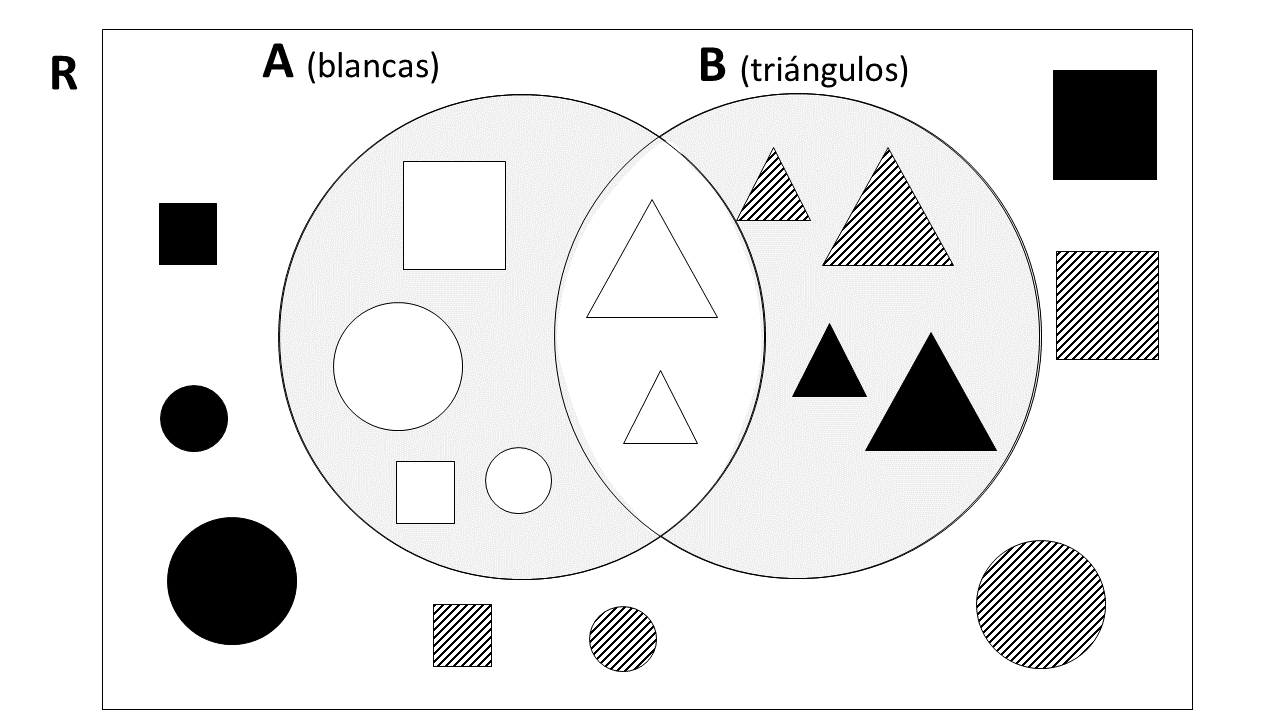
\includegraphics[width=0.5\textwidth]{9b}
\end{figure}
\end{itemize}

\end{enumerate}

%12
\item  \textbf{Ejercicio 11:} Llamemos R a un conjunto referencial cualquiera, $A$ al conjunto de los elementos de R que hacen verdadera la proposición \textbf{p} y $B$ al conjunto de los elementos de R que hacen verdadera la proposición \textbf{q}. Presentamos el cuadro completo:

\begin{table}[ H]
\begin{center} 
\begin{tabular} { l c c l }
\textbf{Proposición}&\textbf{Forma conjuntista}& & \textbf{Representación gráfica}\\ \hline  \\ 

\textbf{p} es Verdadera& A& & 
\begin{minipage}{5cm} 
\begin{center} 
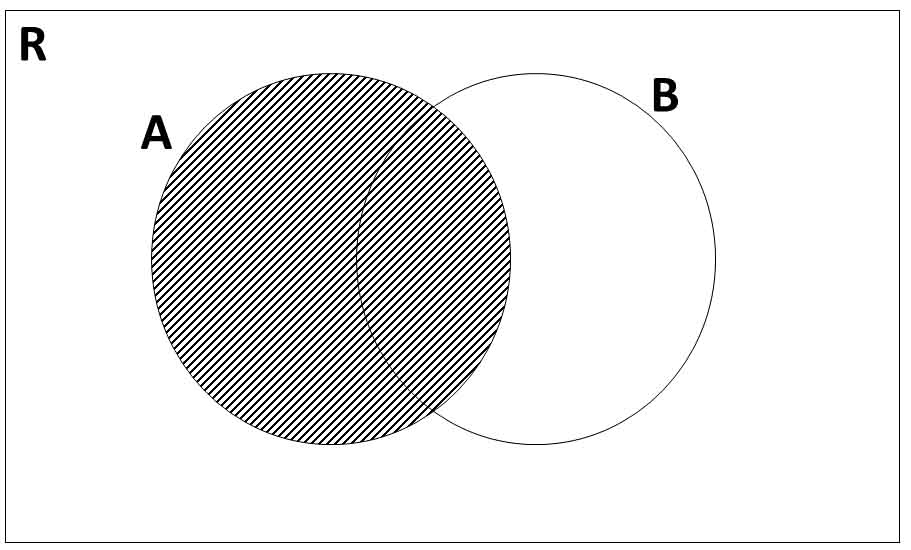
\includegraphics[width=0.6\textwidth]{TP1Fig3.jpg} 
\end{center}
\end{minipage}\\ \\ 

$\textbf{p}$  es F o $\sim p $ es V &$\bar{A}$ & & 
\begin{minipage}{5cm} 
\begin{center} 
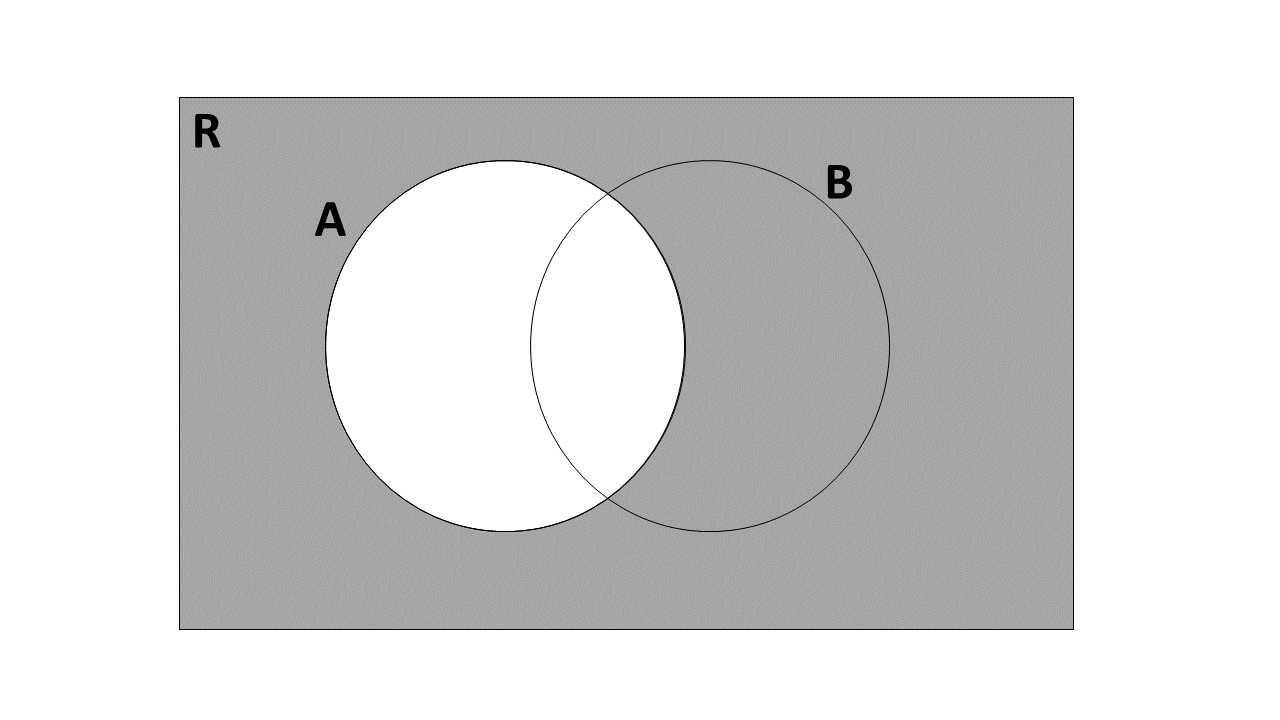
\includegraphics[width=0.8\textwidth]{11a.png} 
\end{center}
\end{minipage}\\ \\   

\end{tabular} 
\end{center} 
\end{table}

\begin{table}[ H]
\begin{center} 
\begin{tabular} { l c c l }
\textbf{Proposición}&\textbf{Forma conjuntista}& & \textbf{Representación gráfica}\\ \hline  \\ 
%\hline
$\textbf{q}$  es F o $\sim q $ es V &$\bar{B}$& & 
\begin{minipage}{5cm} 
\begin{center} 
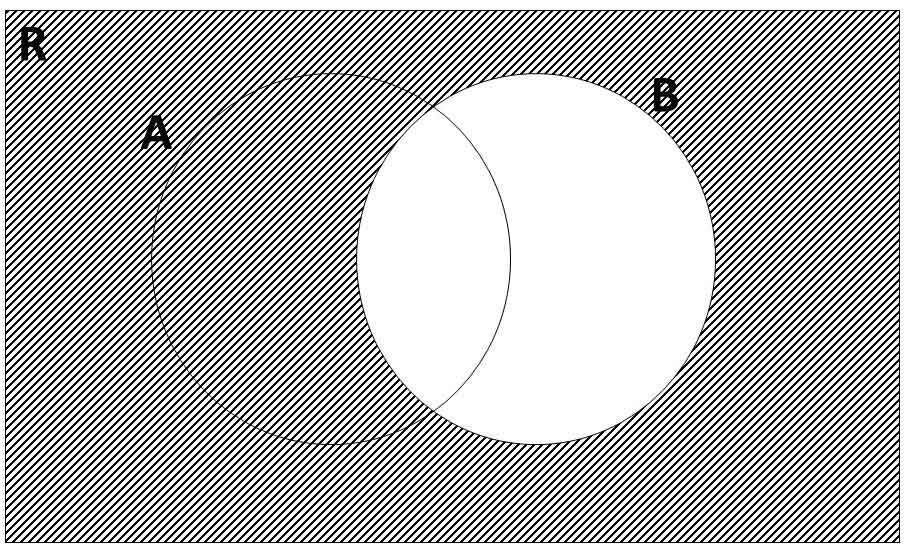
\includegraphics[width=0.6\textwidth]{TP1Fig4.jpg} 
\end{center}
\end{minipage}\\ \\ 

 $p \wedge q$ es V &$A \cap B.$ & &
\begin{minipage}{5cm} 
\begin{center} 
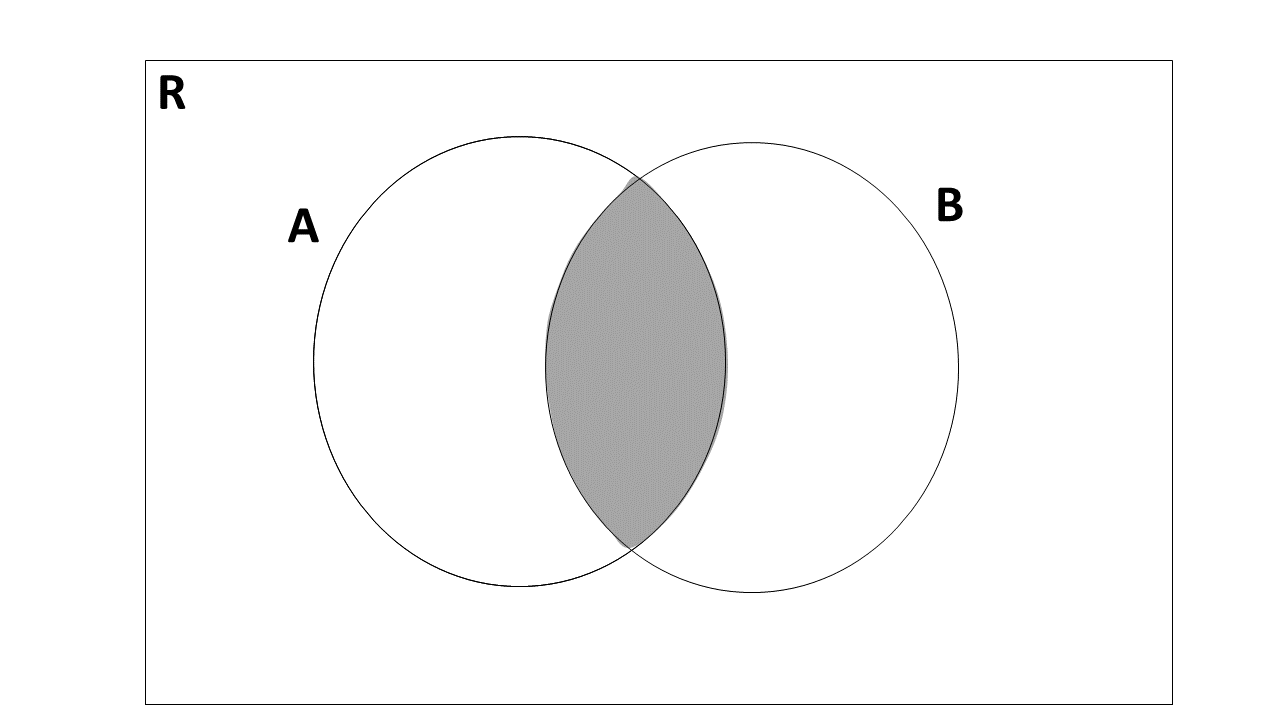
\includegraphics[width=0.8\textwidth]{11b.png} 
\end{center}
\end{minipage}\\ \\  

$\sim p  \vee \sim q$ es V & $\bar{A}\cup \bar{B} = \overline{A\cap B}$ & &
\begin{minipage}{5cm} 
\begin{center} 
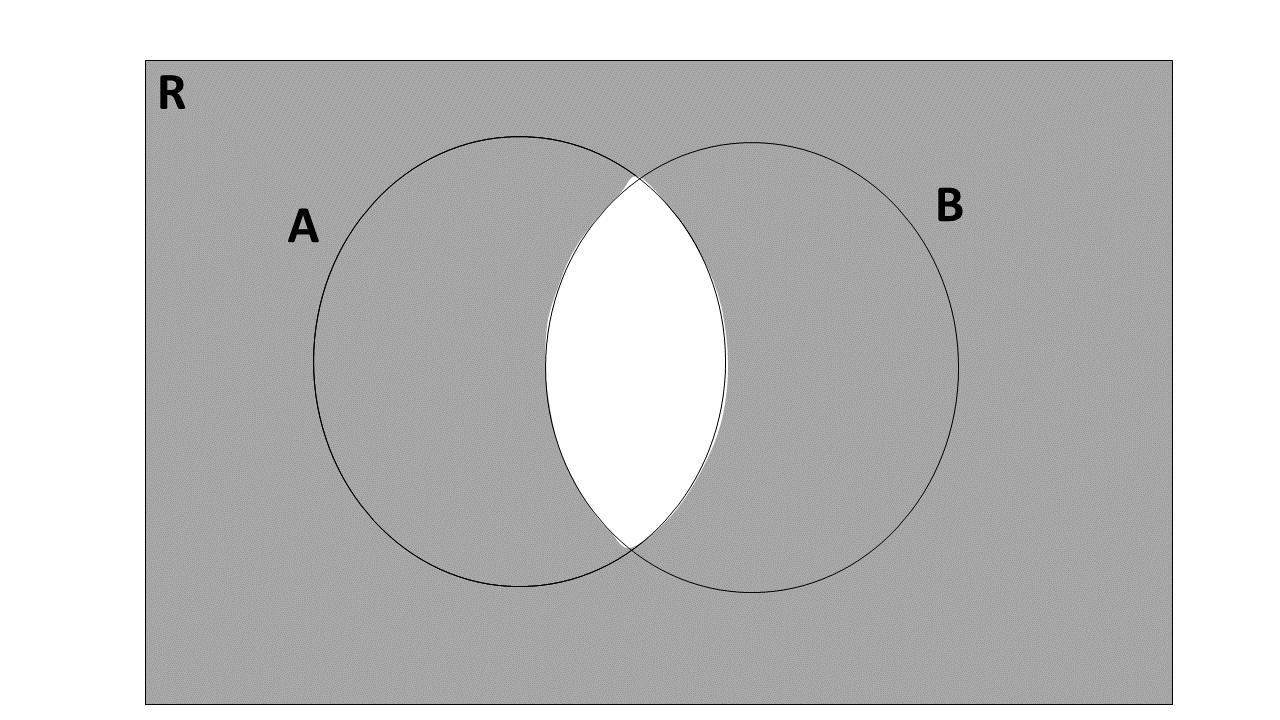
\includegraphics[width=0.8\textwidth]{11c.png} 
\end{center}
\end{minipage}\\ \\

  
$ p \vee q$ &$A \cup B$&  & 
\begin{minipage}{5cm} 
\begin{center} 
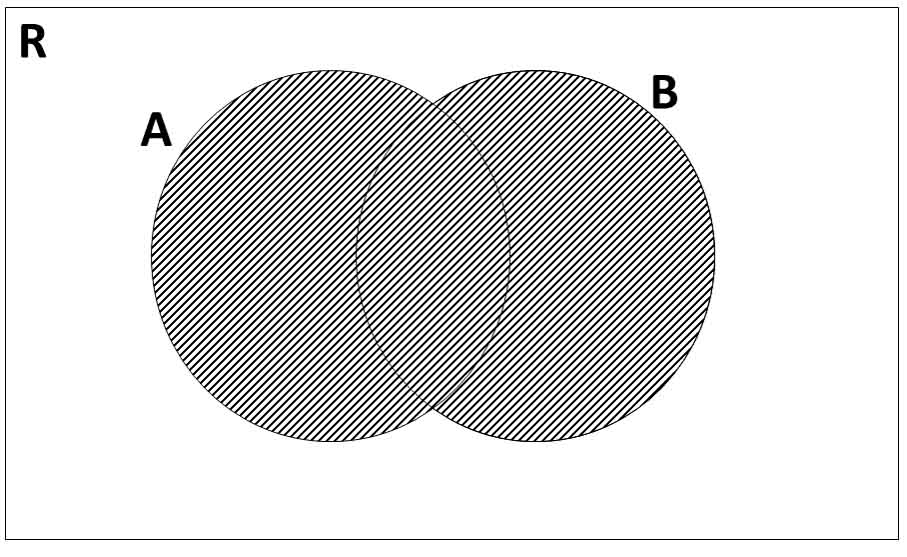
\includegraphics[width=0.6\textwidth]{TP1Fig5.jpg} 
\end{center}
\end{minipage}\\ \\ 

$\sim (p \vee q)$ es V & $\overline{A\cup B}$& & 
\begin{minipage}{5cm} 
\begin{center} 
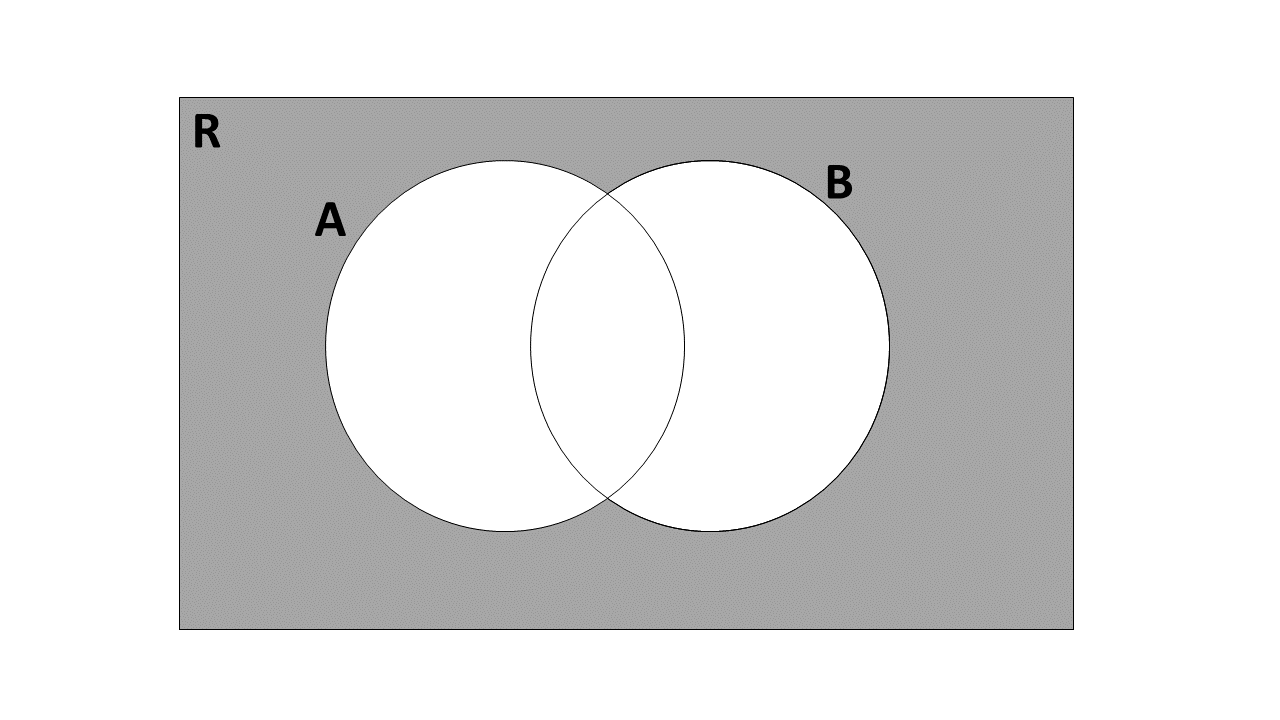
\includegraphics[width=0.8\textwidth]{11d.png} 
\end{center}
\end{minipage}\\ \\   

$ p \wedge \sim q $ &$A-B$ & & \begin{minipage}{5cm} \begin{center} 
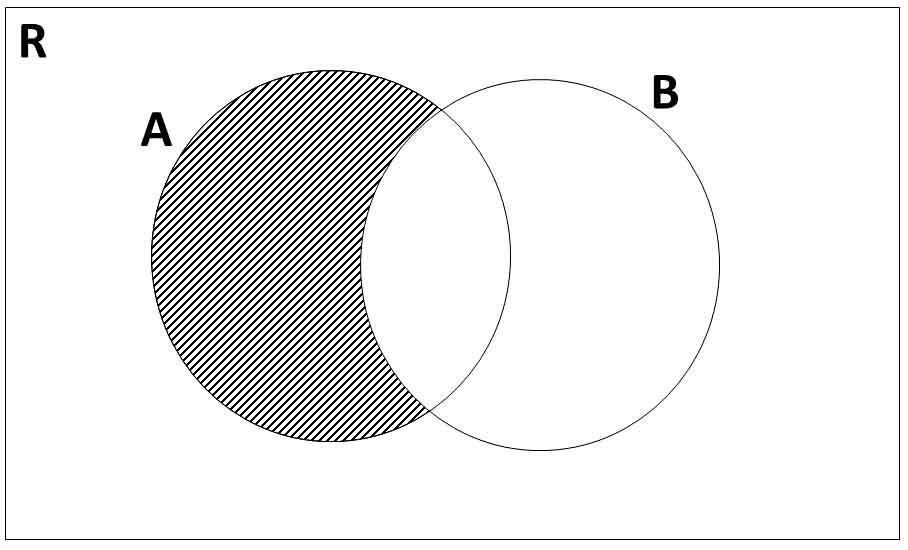
\includegraphics[width=0.6\textwidth]{TP1Fig7.jpg} 
\end{center}
\end{minipage}\\ \\   
$p \veebar q$ &$A \bigtriangleup B = (A \cup B ) - (A \cap B)$ & & \begin{minipage}{5cm} \begin{center} 
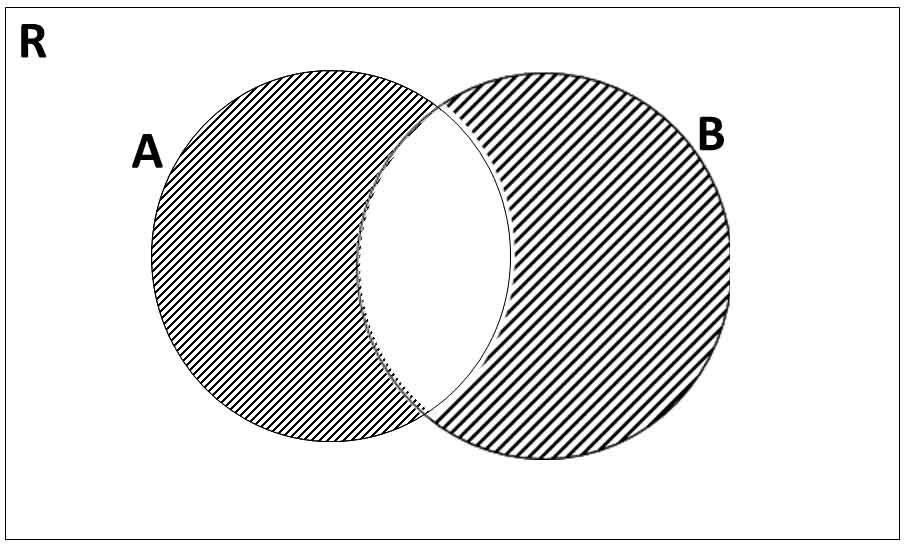
\includegraphics[width=0.8\textwidth]{TP1Fig8.jpg} 
\end{center}
\end{minipage}
\end{tabular} 
\end{center} 
\end{table}


%22
\item \textbf{Ejercicio 17: } En los enunciados siguientes (en el TP están como ejercicio 16), reconocer el antecedente y el consecuente y escribirlos como una implicación. La solución en cada ítem. 
\begin{itemize}
\setlength\itemsep{0em}
\item Para ser investigador de Conicet es necesario haber alcanzado el grado de doctor.\\
\textbf{R:}
%\setlength\itemsep{0em}
El \textbf{antecedente} es: $p$: $x$ (fulano) es  investigador de Conicet. y el   \textbf{consecuente} es: $q$: $x$ es doctor. La implicación $p \Rightarrow q$ puede escribirse de diferentes maneras: 
\begin{itemize}
\item Si $x$ es investigador de Conicet, entonces es doctor.
\item Ser investigador de Conicet implica ser doctor.
\item Ser inverstigador de Conicet es condición suficiente para ser doctor. 
\item Ser doctor es condición necesaria para ser investigadore de Conicet. 
\item Todo investigador de Conicet es doctor. 
\end{itemize}

\item Es necesario ser mayor de edad para emitir un voto electoral.\\
\textbf{R:}
%\setlength\itemsep{0em}
El \textbf{antecedente} es: $p$: $x$ emite un voto, y el   \textbf{consecuente} es: $q$: $x$ es mayor de edad. La implicación $p \Rightarrow q$ puede escribirse de diferentes maneras: 
\begin{itemize}
\item Si $x$ vota, entonces es mayor de edad.
\item Votar implica ser mayor de edad.
\item Votar es condición suficiente para ser mayor de edad. 
%\item Ser doctor es condición necesaria para ser investigadore de Conicet. 
\item Toda persona que vota es mayor de edad. 
\end{itemize}

\item Es necesario ser mamífero para ser ballena.\\
\textbf{R:}
%\setlength\itemsep{0em}
El \textbf{antecedente} es: $p$: $x$ es ballena, y el   \textbf{consecuente} es: $q$: $x$ es mamífero. La implicación $p \Rightarrow q$ puede escribirse de diferentes maneras: 
\begin{itemize}
\item Si $x$ es ballena, entonces es mamífero.
\item Ser ballena implica ser mamífero.
\item Ser ballena es condición suficiente para ser mamífero. 
%\item Ser doctor es condición necesaria para ser investigadore de Conicet. 
\item Toda ballena es mamífero. 
\end{itemize}
\item Es necesario estar inscripto en la carrera Licenciatura en Ciencias Biológicas para cursar Matemática 1 como alumno regular.\\
\textbf{R:}
\setlength\itemsep{0em}
El \textbf{antecedente} es: $p$: $x$ cursa Matemática 1 como alumno regular, y el   \textbf{consecuente} es: $q$: $x$ es está inscripte en la LB. La implicación $p \Rightarrow q$ puede escribirse de diferentes maneras (simplifico la escritura): 
\begin{itemize}
\item Si $x$ cursa M1, entonces está inscripto en la LB.
\item Cursar M1 implica estar inscripto en la LB
\item Cursar M1 es condición suficiente para está inscripto en la LB. 
%\item Ser doctor es condición necesaria para ser investigadore de Conicet. 
\item Toda persona que cursa M1 está inscripta en la LB. 
\end{itemize}
\end{itemize}

\vspace{1.5 cm}

\textbf{Algunos problemas adicionales sobre proposiciones condicionales}

\item \textbf{Ejercicio 24: }Concentremos la atención en aquellas implicaciones que aparecen “ocultas” en el lenguaje coloquial. Consideremos el siguiente ejemplo publicado en un diario:
 
\textit{ “Para cargo gerencial se busca Licenciado en Ciencias Económicas, con referencias comprobables de al menos dos empresas en el ramo, menor de 40 años, con posibilidades de radicarse en la ciudad de Neuquén”.}

Reconocé las proposiciones (simples o compuestas) que forman el antecedente y el consecuente y escribí el aviso en un enunciado de la forma \textit{Si... entonces...} utilizando los conectivos que necesites.

\noindent
\textbf{Solución}\\ 
\textit{Si} la persona $x$ es Licenciada en Ciencias Económicas ($p$) y posee referencias comprobables en al menos dos empresas del ramo ($q$), y tiene menos de 40 años ($r$) y tiene posibilidades de radicarse en la ciudad de Neuquén ($s$), \textit{entonces} $x$ puede aspirar al cargo gerencial de la empresa ($t$). Simbólicamente: $(p \wedge q \wedge r \wedge s) \Rightarrow t$. La proposición compuesta $p \wedge q \wedge r \wedge s$ es el antecedente y la proposición $s$ el consecuente.


%26
\item \textbf{Ejercicio 26: } Cuestiones para pensar en relación a estos dos avisos, para el caso en que las implicaciones sean verdaderas. Para el primer aviso ejercicio anterior, entre otras, estas dos personas pretenden el trabajo:
\begin{itemize}
\item Juan Gómez, Licenciado en Ciencias Económicas, casado, de 43 años de edad con amplia experiencia en empresas del ramo, podría radicarse en Neuquén.
\item Pablo Ramos, Licenciado en Ciencias Económicas y Analista de Sistemas, de 33 años de edad, presenta seis cartas de recomendación de empresas en el ramo, residente en Neuquén. 
\end{itemize}

\begin{enumerate}
\item Juan Gómez ¿puede aspirar al cargo? ¿Por qué?\\
\textbf{R:} No, no cumple con la condición de ser menor de 40 años. Si una de las proposiciones de una conjunción es falsa, lo es toda la conjunción. 

\item Pablo Ramos ¿puede aspirar al cargo? ¿Por qué?\\
\textbf{R:} Si, porque cumple con todos los requisitos (todas las proposiciones del antecedente son verdaderas), aun cuando le sobre.

\item ¿Pablo Ramos obtendrá el cargo?\\
\textbf{R:} No sabemos. Tiene todas las condiciones para aspirar al cargo, puede aspirar. Eso es lo que dice la implicación.

\item Si le dieron a José Ulloa el cargo, ¿qué sabemos de él? (Supongamos que no hay acomodo).\\
\textbf{R:} que, al menos, es Lic. en Ciencias Económicas, posee referencias comprobables en al menos dos empresas del ramo, tiene menos de 40 años y tiene posibilidades dd radicarse en la ciudad de Neuquén.
\end{enumerate}
 
\end{enumerate}
\noindent
\textbf{Bonus} (un ejercicio de un parcial viejo)\\
\noindent
Consideremos ahora los siguientes conjuntos definidos dentro del conjunto referencial de todas las palabras del idioma español:
\begin{itemize}
	\item $A$ el conjunto formado por las palabras de dos sílabas
	\item $B$ el conjunto formado por las palabras terminadas en r
	\item $C$ el conjunto formado los verbos en infinitivo (terminados en ar, er, ir), 
	\item $D$ el conjunto formado por los nombres comunes de animales (perro, caballo, tapir, saltamontes,…), 
	\item $E$ el conjunto formado por las palabras terminadas en s, 
	\item $F$ el conjunto formado por las palabras con tilde en la última sílaba (camión, además) (Acordarse de que las palabras agudas (acentuadas en la última sílaba) sólo llevan tilde si terminan en n, s o vocal. Por ejemplo camión lleva, vocal no lleva)
\end{itemize}
\begin{enumerate}
	\item Representar estos conjuntos usando diagramas de Venn\\
		\begin{figure}[H]
		\centering
		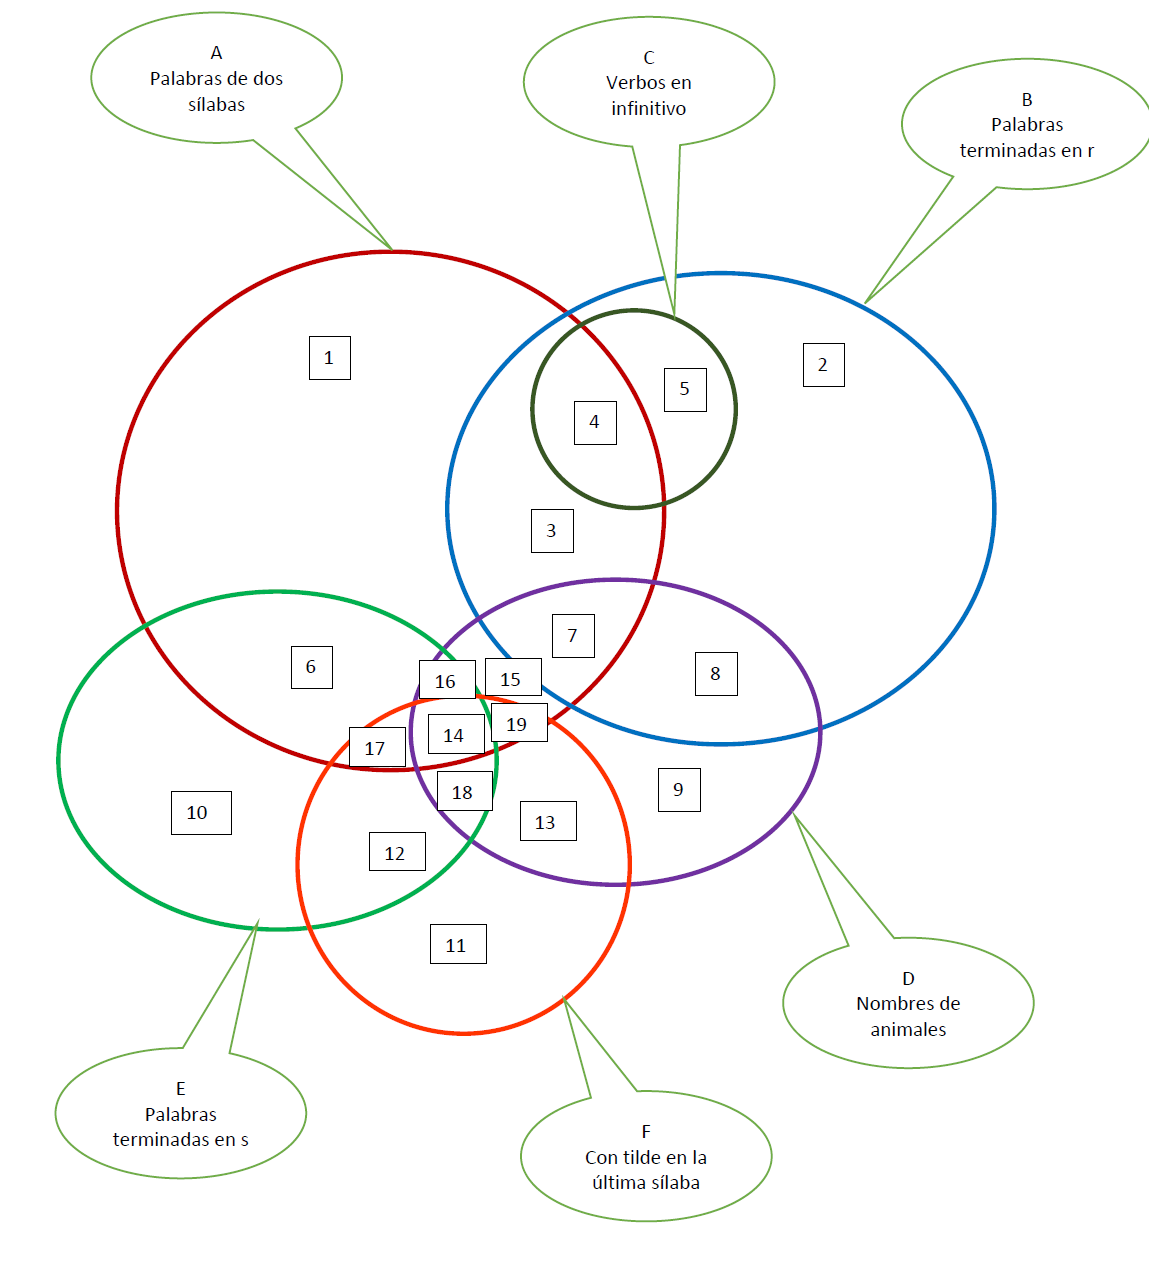
\includegraphics[width=0.7\textwidth]{bonus.png}
		\end{figure}
	\item Poner un ejemplo en cada región determinada en el gráfico\\
	\textbf{R:} Sólo se pedían los ejemplos, pero pongo de qué se trata cada región para ayudar a pensar los ejemplos.
		\begin{itemize}
		\item 1. Palabras de dos sílabas que no terminan en r, no son nombres de animales, no terminan en s y no tienen tilde en la última sílaba. Ejemplo: casa
		\item 2. Palabras terminadas en r que no son verbos en infinitivo, no tienen dos sílabas, no son nombres de animales. Ejemplo: automotor
		\item  3.Palabras de dos sílabas terminadas en r que no son verbos en infinitivo. Ejemplo: motor
		\item  4. Verbos en infinitivo (y consecuentemente terminados en r) que tienen dos sílabas. Ejemplo: saltar.
		\item  5. Verbos en infinitivo (y consecuentemente terminados en r) que no tienen dos sílabas. Ejemplo: caminar
		\item  6. Palabras de dos sílabas que terminan en s, no son nombres de animales ni tienen tilde. Ejemplo: alas
		\item 7. Nombres de animales que terminan en r y tienen dos sílabas. Ejemplo: castor
		\item 8. Nombres de animales que terminan en r y no tienen dos sílabas. Ejemplo: calamar
		\item  9. Nombres de animales que no terminan en r, no tienen tilde en la última sílaba, no terminan en s y no tienen dos sílabas. Ejemplo: caballo
		\item 10. Palabras terminadas en s que no tienen dos sílabas, no tienen tilde en la última sílaba y no son nombres de animales. Ejemplo: abrelatas
		\item 11. Palabras con tilde en la última sílaba, no terminan en s, no son nombres de animales ni tienen dos sílabas. Ejemplo: ecuación
		\item 12. Palabras con tilde en la última sílaba, que terminan en s, pero no son nombres de animales ni tienen dos sílabas. Ejemplo: autobús
		\item 13. Palabras con tilde en la última sílaba, que son nombres de animales, pero no terminan en s, ni tienen dos sílabas. Ejemplo: camaleón
		\item 14. Palabras con tilde en la última sílaba, que terminan en s, que son nombres de animales y tienen dos sílabas. Ejemplo: ciempiés.
		\item 15. Palabras que son nombres de animales, tienen dos sílabas pero no terminan en r ni en s y no llevan tilde en la última sílaba. Ejemplo: vaca
		\item 16. Palabras de dos sílabas que no tienen tilde en la última sílaba, que son nombres de animales pero que no terminan ni en s ni en r. Ejemplo: orca
		\item 17. Palabras de dos sílabas terminadas en s, con tilde en la última sílaba que no son nombres de animales. Ejemplo: quizás
		\item 18. Palabras terminadas en s, que llevan tilde en la última sílaba y son nombres de animales, pero no tienen dos sílabas. Ejemplo:
		\item 19. Palabras que tienen tilde en la última sílaba, son nombres de animales, tienen dos sílabas, pero no terminan en s. Ejemplo: león.
		\end{itemize}

	\item Escribir las proposiciones que hacen verdaderas los elementos de  $A \cap C$, $A \cup E$  y  $B -  A$.\\
	\textbf{R:} 
		\begin{itemize}
		\item $A \cap C$: Palabras de dos sílabas y que terminan en r. Ejemplo: soñar
		\item $A \cup E$: Palabras de dos sílabas o terminadas en s. Ejemplos: casa, malezas, pares
		\item $B -  A$: Palabras terminadas en r y que no tienen dos sílabas. Ejemplo: aprobar
		\end{itemize}
	\item Escribir una implicación verdadera (de la forma \textit{Si... entonces...}) que puedan efectuarse en relación a las proposiciones que inducen los conjuntos $A$ a $F$. \\
	\textbf{R:} Pongo un ejemplo, hay muchos:
		\begin{itemize}
		\item Si (la palabra $x$) es un verbo en infinitivo, entonces es una palabra terminada en r. (porque $C \subset B$)
		\item Si (la palabra $x$) es una palabra terminada en s entonces no es una palabra terminada en r ($D \subset  \bar{B}$)
		\end{itemize}
	\item Escribir una afirmación verdadera que contenga el cuantificador \textit{Todo} y otra que contenga el cuantificador \textit{Existe}(en relación a los conjuntos propuestos).
	\textbf{R:} 
		\begin{itemize}
		\item \textit{Todo} verbo en infinitivo, es una palabra terminada en r
		\item \textit{Existe} una palabra de dos sílabas que es un nombre de animal
		\end{itemize}
	\item Expresar la negación lógica de las afirmaciones escritas en el inciso e)  (obviamente falsas).\\
	\textbf{R:} 
		\begin{itemize}
		\item \textit{Existe} un verbo en infinitivo que no es una palabra terminada en r
		\item \textit{Toda} palabra de dos sílabas no es un nombre de animal
		\end{itemize}

\end{enumerate}

\end{document}
